\subsubsection{Kopfbeleuchtung}
\label{subsubsec:led}

Die \gls{led}-Reihen an den beiden Außenseiten des Kopfes sind, wie in Kapitel \ref{sec:roboterarchitektur-und-systemkomponenten}
beschrieben, am Jetson Nano des Kopfes angeschlossen.
Prüft man dort die Funktionen, die über den Autostart gesteuert werden, so fallen zwei Ordner auf - \texttt{faceLightServer/}
und \texttt{faceLightMqtt/}.
Leider sind die Funktionalitäten beider Skripte als Binärdateien abgelegt und somit nicht ohne weiteres auslesbar.
Auch die Dokumentation des Herstellers weist keinerlei Informationen zu den \gls{led}-Reihen auf.
Der Name des zweiten Ordners weist jedoch auf eine mögliche Funktionalität der Steuerung über MQTT hin.
Um dies zu bestätigen, lässt sich ein MQTT-Explorer verwenden.
Dieser registriert sich als Client beim MQTT-Broker und schreibt alle Nachrichten und veröffentlichten Topics mit.
Mehr zum Thema MQTT gibt es auf der offiziellen Dokumentation des Standards\footnote{https://mqtt.org/} und in Kapitel \ref{sec:funktionserweiterungen-und-integration}.

Zur Nutzung des MQTT Explorers wird die \gls{ip} Adresse des Brokers und der Port, auf dem dieser veröffentlicht wird, benötigt.
Für die Adresse kommen nur die \glspl{ip} \texttt{192.168.123.13}, \texttt{...14}, \texttt{...15} und \texttt{...161}
infrage.
Es kann mit der Bibliothek \emph{Nmap} geprüft werden, ob der MQTT-Standardport \texttt{1883} auf einer der registrierten \glspl{ip}
im Netz \texttt{192.168.123.0/24} geöffnet ist.

\begin{lstlisting}[language=Bash]
nmap -sS -O -p1883 192.168.123.0/24
\end{lstlisting}

\noindent Die Ausgabe zeigt, dass die beiden \glspl{ip}
\texttt{192\allowbreak .168\allowbreak .123\allowbreak .15} und \texttt{192\allowbreak .168\allowbreak .123\allowbreak .161} den MQTT Port offen haben.
Über den MQTT Explorer wird zunächst der NVIDIA Jetson Xavier NX als Broker getestet.
Die Verbindung funktioniert, jedoch werden weder verfügbare Topics noch Messages ausgegeben.
Ein Test auf dem Raspberry Pi mit der \gls{ip} \texttt{192.168.123.161} zeigt die Ausgabe wie in Abbildung \ref{fig:mqtt-explorer}
dargestellt.

\begin{figure}[h]
    \frame{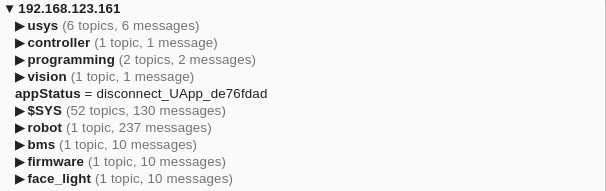
\includegraphics[width=\linewidth]{img/analyse/mqtt-explorer}}
    \caption{Ausgabe eines MQTT Explorers in Verbindung mit dem Raspberry Pi als Broker}\label{fig:mqtt-explorer}
\end{figure}

\noindent Auffällig ist hier das Topic \texttt{face\_light/\allowbreak color}, welches in reg
% todo auf schorsch connecten, rocky ist bereits geändert, format herleiten, doku suchen

